\documentclass[11pt]{article}
\usepackage[a4paper, portrait, margin=1in]{geometry}
\usepackage{graphicx}
\usepackage{listings}
\usepackage{epstopdf}
\usepackage{caption}
\usepackage{svg}
\usepackage{amsmath}
\usepackage{lscape}

\begin{document}

\newsavebox\IBoxA \newsavebox\IBoxB \newsavebox\IBoxC \newlength\IHeight
\newcommand\TriFig[9]{% Image1 Caption1 Label1 Image2 ...
	\sbox\IBoxA{\includegraphics[width=0.32\textwidth]{#1}}
	\sbox\IBoxB{\includegraphics[width=0.32\textwidth]{#4}}
	\sbox\IBoxC{\includegraphics[width=0.32\textwidth]{#7}}%
	\ifdim\ht\IBoxA>\ht\IBoxB
	\setlength\IHeight{\ht\IBoxB}\else\setlength\IHeight{\ht\IBoxA}\fi%
	\ifdim\ht\IBoxA>\ht\IBoxC
	\setlength\IHeight{\ht\IBoxC}\else\setlength\IHeight{\ht\IBoxA}\fi%
	\ifdim\ht\IBoxB>\ht\IBoxC
	\setlength\IHeight{\ht\IBoxC}\else\setlength\IHeight{\ht\IBoxB}\fi%  
	\begin{figure}[!htb]
		\minipage[t]{0.32\textwidth}\centering
		\includegraphics[height=\IHeight]{#1}
		\caption{#2}\label{#3}
		\endminipage\hfill
		\minipage[t]{0.32\textwidth}\centering
		\includegraphics[height=\IHeight]{#4}
		\caption{#5}\label{#6}
		\endminipage\hfill
		\minipage[t]{0.32\textwidth}\centering
		\includegraphics[height=\IHeight]{#7}
		\caption{#8}\label{#9}
		\endminipage
	\end{figure}%
}

\newcommand\TwoFig[6]{% Image1 Caption1 Label1 Image2 ...
	\sbox\IBoxA{\includegraphics[width=0.55\textwidth]{#1}}
	\sbox\IBoxB{\includegraphics[width=0.55\textwidth]{#4}}%
	\ifdim\ht\IBoxA>\ht\IBoxB
	\setlength\IHeight{\ht\IBoxB}\else\setlength\IHeight{\ht\IBoxA}\fi%
	\begin{figure}[!htb]
		\minipage[t]{0.5\textwidth}\centering
		\includegraphics[height=\IHeight]{#1}
		\caption{#2}\label{#3}
		\endminipage \hfill
		\minipage[t]{0.5\textwidth}\centering
		\includegraphics[height=\IHeight]{#4}
		\caption{#5}\label{#6}
		\endminipage
	\end{figure}%
}


\title{Advanced Systems Lab (Fall'15) -- First
Milestone}

\author{Name: \emph{Sandro Huber}\\Legi number: \emph{10-924-777}}

\date{
\vspace{4cm}
\textbf{Grading} \\
\begin{tabular}{|c|c|}
\hline  \textbf{Section} & \textbf{Points} \\ 
\hline  1.1 &  \\ 
\hline  1.2 &  \\ 
\hline  1.3 &  \\ 
\hline  2.1 &  \\ 
\hline  2.2 &  \\ 
\hline  2.3 &  \\ 
\hline  3.1 &  \\ 
\hline  3.2 &  \\ 
\hline  3.3 &  \\ 
\hline  3.4 &  \\ 
\hline  3.5 &  \\ 
\hline  3.6 &  \\ 
\hline \hline Total & \\
\hline 
\end{tabular} 
}

\maketitle

\newpage

\section{System Description}\label{sec:system-description}

\subsection{Database}\label{sec:database}

Length: 1-2 pages

Start by explaining the schema of the database and the indexes used to
speed up data access. Describe the interface to the database (queries
and stored procedures).

Make sure to explain the design in terms of what you wanted to achieve,
what decisions you took and what is the expected behavior.

Include baseline performance characteristics of the database (max
throughput, response time, and scalability).

\subsubsection{Schema and Indexes}\label{sec:schema-and-indexes}
\begin{figure}[!ht]
\centering
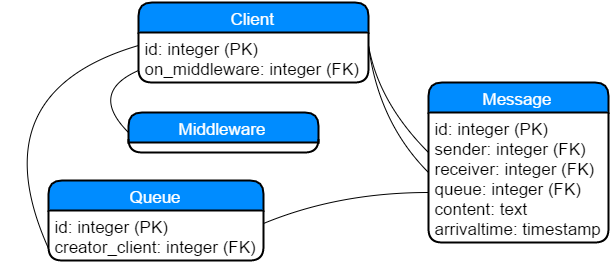
\includegraphics[width=0.7\linewidth]{figures/database/db_schema}
\caption{The Database Schema}
\label{fig:db_schema}
\end{figure}
The database schema was chosen in such a way, that it provides all required functionality, but is still easy to setup and maintain. The following lines shortly illuminate the tables and their column types.
\begin{itemize}
	\item \textbf{Client}: Guarantees through the serial datatype that each client in the whole system has a unique ID and stores which client is registered on which middleware. This can be handy when wanting an even distribution of clients over all middlewares.
	\item \textbf{Queue}: Stores all queues created by clients. Also ensures that all queues are unique.
	\item \textbf{Middleware}: A sequence which is used to get a unique ID for each middleware joining the system.
	\item \textbf{Message}: Here, all messages sent by clients are stored. The foreign keys ensure that we only get messages from valid clients registered in the system. As one can see, the content column is of type text, despite the choice of varchar(200) or varchar(2000) may be more obvious with respect to the system requirements. Find my thoughts about this choice in section \ref{sec:design-decisions}.
\end{itemize}
To speed up the data access I used the two following indices:
\begin{lstlisting}[language=SQL,basicstyle=\small]
(a) INDEX msg_rcvr_q_idx ON MESSAGE (RECEIVER, QUEUE);
(b) CREATE INDEX msg_sndr_idx ON MESSAGE (SENDER);
\end{lstlisting}
The reasoning behind the choice of them is based on the following thoughts. The indices in a database system affect search time, i.e. filtering of rows with respect to a criterion. Since the whole system is built with predefined stored procedures (find a full list in section \ref{sec:stored-procedures}) we know exactly what these filter parameters will be. To simplify the view, only the most relevant parts of the queries are shown (query they belong to in brackets):
\begin{lstlisting}[language=SQL,basicstyle=\small,escapeinside={(*@}{@*)}]
(1) WHERE RECEIVER (*@(get\_queues\_for\_client)@*)
(2) WHERE RECEIVER AND QUEUE (*@(read\_all\_messages\_of\_queue)@*)
(3) WHERE RECEIVER AND QUEUE ORDER BY ARRIVALTIME (*@(remove\_top\_message\_from\_queue)@*)
(4) WHERE RECEIVER AND SENDER ORDER BY ARRIVALTIME (*@(read\_message\_from\_sender)@*)
\end{lstlisting}
Since an index on two columns (c1, c2) is also an index onto c1, we can see that the index (a) already covers the WHERE clauses of (1)-(3). In addition with index (b) we get a full coverage of all queries having to filter some data. It is intentional that there is no index on the GROUP BY of ARRIVALTIME. Find more about the reasoning in section \ref{sec:design-decisions}.

\subsubsection{Stored Procedures}\label{sec:stored-procedures}
Every database access is done via a stored procedure. This allows to have a single point of failure, maintenance and control over functionality. Having this lone entry guarantees fast and reliable feature implementation and debugging. In Java the stored procedures are interfaced via Prepared Statments, which can be cached by the VM, such that only the dynamic parameter values have to get fetched, before a query can be executed. The following stored procedures are implemented:
\begin{lstlisting}[basicstyle=\small]
create_queue(creator_client INTEGER)
delete_queue(queue_id INTEGER)
register_client(on_middleware INTEGER)
get_queues_for_client(client_receiver INTEGER)
read_all_messages_of_queue(receiver_id INTEGER, queue_id INTEGER)
read_message_from_sender(sender_id INTEGER, receiver_id INTEGER)
remove_top_message_from_queue(receiver_id INTEGER, queue_id INTEGER)
send_message(sender_id INTEGER,
	receiver_id INTEGER, queue_id INTEGER, content TEXT)
register_middleware()
get_registered_clients()
get_number_of_messages()
get_registered_queues()
take_stamp()
\end{lstlisting}

\subsubsection{Design decisions}\label{sec:design-decisions}
The design aims to be simple, but yet complex enough to provide all necessary functionalities through a nice interface. Please find in the following lines the reasoning about some design decision I took while implementing the system:
\begin{itemize}
	\item \textbf{text vs varchar(n)}: First of all, all datatypes char(n), varchar(n), varchar and text are internally all converted to the same C data structure varlena. So from the performance perspective no (major) differences are measurable. Because I wanted to be flexible and send messages of length 200 and 2000 in the same setup I decided to go with the flexible variant text. Choosing varchar(2000) for every case is bad, because the unused space when inserting smaller strings will be filled with spaces and thus not give any performance advantages.
	\item \textbf{Ghost-Client}: Since messages can also be addressed to all clients in the system, I introduced a ghost-client with an ID of 0, which gets created right at the database initialization. This ghost-client allows that instead of having RECEIVER=NULL, we have RECEIVER=0 for all broadcast messages, which is internally much easier to handle.
	\item \textbf{Index on ARRIVALTIME}: Maintaining an index is not cheap for a database system, so it's wise to use them with caution. Because of that I decided that the indices (1) and (2) are already discarding enough rows, such that the sorting operation is not too costly anymore.
	\item \textbf{ARRIVALTIME location}: The ARRIVALTIME is implemented as a trigger on the database. Another, also valid choice, would have been to let the client set it. But because I wanted to minimize the work of the clients and guarantee a unique timestamp on each message I did choose the trigger-option.
\end{itemize}

\subsubsection{Performance characteristics}\label{sec:performance-characteristics}
To measure the performance of the database I used the postgresql tool pgbench. For the machine details, please refer to section \ref{sec:system-configurations}. I defined three levels of difficulty, which correspond to different query sets, level 0 beeing the easiest, level 2 the hardest. This allows us to get a smooth transition from absolute best to real-world behaviour. For a detailed insight into the levels, please find them in /db\_baseline/benchScripts. All contents had length 200. Before running the presented experiment I tested how many clients per database connection are optimal. I expected that the relation of 1:1 should hold, which indeed was the case. For the throughput and latency I expect the knee to be found around 16 clients, because we work with a machine that provides 8 physical cores and the official rule of thumb given in the PostgreSQL documentation\footnote[1]{https://wiki.postgresql.org/wiki/Number\_Of\_Database\_Connections} is \textit{optimal number of DB connections} $\approx$ $2(core\_count)+c$, where $c$ is a constant. Of course the throughput level ranking from hightest to lowest should be: 0, 1, 2+, 2- (+/- for with or without indices), and vice-versa with the latency. After the knee there should at least be a visible stagnation of the throughput, but a remarkable increase of latency.
\TwoFig {figures/database/levels0_2_tp.eps} {Database Throughput} {fig:tp}
		{figures/database/levels0_2_lat.eps} {Database Latency} {fig:lat}

Firstly please note, that the lack of data around 30 clients is explained through a bug in the code. But it does not seem that any exceptional behaviour is missed due to that. As one can see (the lines follow the 50\% quantiles), the knees can really be found around the expected 16 clients. Also the rank of the levels behave as expected. I am especially happy about the performance benefit gained by the indices. Only the gain of latency after the barely visible knee is not as steep as foreseen. But this is probably okay, since we can't see a total throughput breakdown neither. The most costly operation in the whole benchmark is identified as the removal of the top message, i.e. executing \textit{remove\_top\_message\_from\_queue}. To further investigate this I performed the subsequent follow-up experiment.

The speed of the top most message removal is highly correlated with the size of the database, because the more messages, the longer the index access and the longer the sorting (ORDER BY) of the final table entries will take. To simulate an extreme scenario I only registered one client and one queue in the system into which all messages were sent. All messages also had sender and receiver set to the lone client and had a random content of length 200. This allows to focus on the behaviour of the performance of the query with respect to the size of the database. The database was benched by 40 concurrent clients (for machine type reference, please look up section \ref{sec:system-configurations}), operating on 40 database connections. I chose 40, because we just saw, that around this many clients, the database throughput on the level 2+ was maximal. Each client ran independantly and chose randomly between either inserting 10 new messages, or removing the top most message of the single queue 3000 times. This workload ensured, that the database grows over time and the whole experiment runs sufficiently long. According to the behaviour in the last experiment I expect a steady increase of the latency, following the trend of the database size quite closely.
\begin{figure}[!htb]
\centering
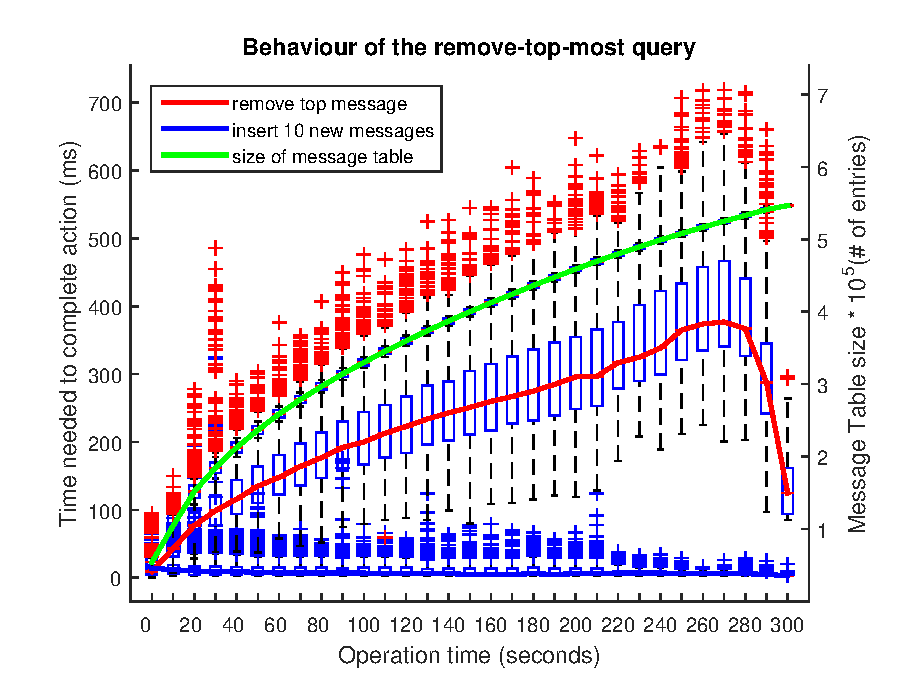
\includegraphics[width=0.7\linewidth]{figures/database/data_baseline}
\caption*{}
\label{fig:data_baseline}
\end{figure}
It's clearly visible that the expectation of having a close relation between the performance of the query and the database size is true. To be sure, that the insertion of new messages does not blur the picture, also this data is plotted. The abrupt break-down of the latency at the end of the experiment is due to the completion of the first few clients. This allows the ones still running to get a congestion-free access to the database. It is visible, that the database stays stable, even when going up to half a million entries in the message table.


\subsection{Middleware}\label{sec:middleware}

Length: 1-2 pages

Explain the design from a high-level point of view, highlighting what
you wanted to achieve, design decisions, expected behavior.

Then go into more detail on how the middleware connects to the database
and clients, and how queuing is implemented.

Show what are the performance characteristics of the middleware
(i.e.~throughput, latency, scalability).

\subsubsection{Design overview}\label{sec:design-overview}
\begin{figure}[!htb]
\centering
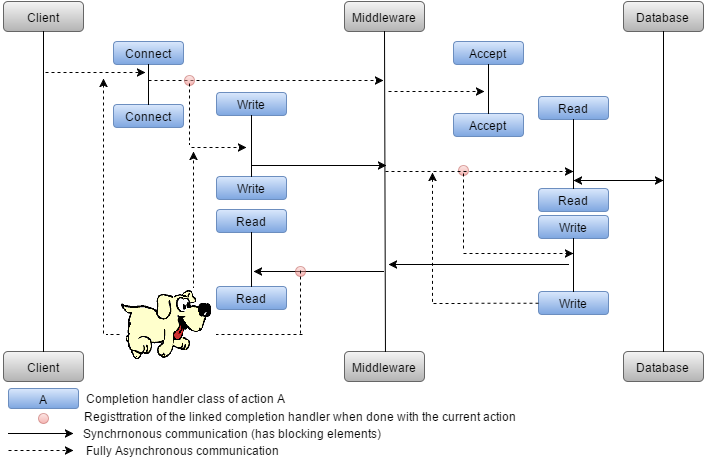
\includegraphics[width=1.0\linewidth]{figures/middleware/mw_design}
\caption{A flow diagram of the whole system, showcasing the completion handler functionality. On the middleware there is a watchdog monitoring all connections, and closing them, when they were inactive for a given time interval. Yet unfinished clients would then have to reconnect.}
\label{fig:mw_design}
\end{figure}
The middleware was designed with the aim to be run fully asynchronous when communicating and be as adaptive as possible to incoming traffic. Initially I was driven by the idea of HTTP: Having a stateless protocol, and each reqeust requires a new connection. This might be nice in theory, but sadly didn't work for this type of project. Although opening a TCP socket connection is instant, closing is not. It resides in a wait state for (on windows) 30 seconds. When having around 100 clients, all sending what they can, my local system blew up around 180'000 open TCP connections, because the operating system ran out of file descriptors. That's why, there is one TCP connection per client. The whole project is based on the NIO-library of Java. It does allow to have a highly modular implementation with respect to the three main tasks, connection establishment, reading and writing of data. The only synchronized parts in the whole design are the sending and writing of messages, such that we can ensure that the whole request is fully sent, before returning the thread to the threadpool. Speaking of the threadpool, I did choose to work with a so called \textit{cached thread pool}. This is a dynamic, i.e unbounded thread pool, which gives the system as many threads as it needs. This is especially useful in our scenario, because we have a lot of small parallel working tasks. There is only one problem, namely deadlocks. Since in the worst case, for every read and write a blocking call is made, it's possible that all threads wait on each-other. To circumvent this, we luckily don't have to do anything. The JVM already manages a second, hidden thread pool, which takes care of all I/O operations on the asynchronous channels. This ensures, that our system is always able to react to new incoming traffic. I expect the middleware to behave stable for at least 32 concurrent clients, since we are operating with 16 hyperthreads (more machine details found in section \ref{sec:system-description}) and one hyperthread should surely be able to deal with two concurrent completion handlers.

\subsubsection{Interfacing with clients}\label{sec:interfacing-with-clients}
The interface between the clients and the middleware has two aspects: A technical and an architectural. From the technical perspective, the interface is provided through a socket and the (IP, port)-tuples. When starting up, each client parses the predefined IP and port number from a config file (see /config/config\_common.xml). Then the socket connection is opened and either closed by the client when it is done with it's job list, or by the watchdog operating on the middleware. The watchdog thread monitors all established connections and surveys activity among all connections in a fixed frequency. If one was idle for too long it get's closed right away. Thus the client may be needed to reconnect in order to send further requests (see Figure \ref{fig:mw_design}). From an architectural point of view, the interface is given through the abstract class Request, which implements the Serializable interface. Depending on the request type of the client, a different subclass, e.g. \textit{CreateQueueRequest} is sent. The overwritten methods \textit{processOnMiddleware} and \textit{processOnClient} define the behaviour of each side for this type of message. The answer sent back to the client is the same type of subclass. Just this time, the fields are set to the answers gotten from the database query. If an error happened, the \textit{exception} field is set, and thus an easy nullity test is required such that the client knows if everything went well.
The following request classes are defined:
\begin{lstlisting}[basicstyle=\small]
CreateQueueRequest
DeleteQueueRequest
GetNumberOfMessagesRequest
GetQueuesWithMessagesForClientRequest
GetRegisteredClientsRequest
GetRegisteredQueuesRequest
HandshakeRequest
ReadAllMessagesOfQueueRequest
ReadMessageFromSenderRequest
RemoveTopMessageFromQueueRequest
SendMessageRequest
RegisterMiddlewareRequest
\end{lstlisting}
For every of these requests there is a corresponding exception class, which caries an informative string that explains the cause of the error.

\subsubsection{Queuing and Connection pool to database}\label{sec:queuing-and-connection-pool-to-database}
When the middleware does start up, it also initializes a connection pool with open JDBC connections to the PostgreSQL database. The (IP, port)-tuple to reach the database as well as the number of concurrent database connections is again fetched from the config file found in \textit{/config/config\_common}. It's important to mention that the connections to the database are only established once in the initialization and from then on reused for the whole life of the middleware and all client requests. The connection pool uses the facility of the \textit{LinkedBlockingQueue} of Java, especially the behaviour on the \textit{take} method: When there are connections available, the queue is not empty and the \textit{take} call instantly pops a connection from the queue, which will be used for the database access. If currently all connections are in use, the call to \textit{take} will block. When a connection now is returned to the pool, the \textit{LinkedBlockingQueue} internally fires a signal, which wakes a random waiting thread in the \textit{take} method up, which is allowed to proceed. This means that there is no fairness and we are not able to guarantee that a thread does not have to wait for a long time before getting a connection. Because the worst thing that can happen is, that the variance is enlarged, I decided that (as long as further experiments don't show a much worse behaviour) this is not a problem.

\subsubsection{Performance characteristics}\label{sec:performance-characteristics-1}
To measure the performance baseline for the middleware I again tried to analyze the Unit-Under-Test (UUT) as isolated as possible. In the case of the middleware this means to fully exclude the database access, but of course not the connection pooling. To generate the work load another machine, running the clients, is used. This setup of course suffers from network latency, but since we are only interested in the within-middleware response time, as long as the network bandwidth is not the bottleneck we're fine. To verify that this is indeed true, before running the main experiment a bandwidth measurement was done, which resulted in a 95\% confidence interval of $\pm15.73$MB/s $(=4.64\%)$ around 339.7 MB/s. Each measurement was performed by sending 5GB of data over the network as fast as possible. There was difference between sending the data in one big packet, or in small 1024kB blocks. This is due to the operating system which does cut the network traffic in small packets anyway. For more insight, please find the scripts for this experiment in \textit{/conn\_throughput\_baseline}. All requests sent in the upcoming experiment use a content size of 200, this makes each request about 2kB big after the serialization. So what can we expect from the middleware? Because of the arguments pointed out in section \ref{sec:design-overview} and section \ref{sec:queuing-and-connection-pool-to-database}, we can expect the system to be stable up to probably 40 clients, before the throughput breaks down and the latency increases significantly.
\TwoFig {figures/middleware/mw_throughput.eps} {Middleware Throughput} {fig:mw_tp}
{figures/middleware/mw_latency.eps} {Middleware Latency} {fig:mw_lat}

Let's first consider only the blue curves (1CM = 1 client machine), i.e. the setting where the middleware was fed by a single client machine. We can clearly see, that the performance of the middleware was underestimated with respect to the number of concurrent clients can get served while still running stably. But after around 60 clients there is a sudden decrease. There can be two causes for this behaviour: (1) the middleware reached it's capacity, or (2) the client is the bottleneck and too many clients are trying to send on the same client machine and hinder each other to run at full capacity. To find if (1) or (2) was the reason for this measurements I introduced a second client machine and ran the upcoming follow-up experiment.

Each client machine only handles half the clients. This ensures that the requests per time unit entering the middleware should at least be the same compared to the single-machine case. Now let's inspect the resulting green curves (2CM = 2 client machines). Indeed it can be verified, that the bottleneck was at the client-side. This can be said, because the throughput from 70 clients on is now stabilized with a small variance, whereas in the latter case we measured a major break-down with high instability. Having a stable throughput and simultaneously an increasing latency is a clear sign, that the performance peak of the middleware was found, in this case at around 70 clients while processing 45'000 requests per second with a response time of $\approx1$ms on average! This is clearly more than expected. The reason for this is that I underestimated the power ob the observer pattern behind the completion-handler-system. But one question the plot poses is not yet asked: Why is the throughput for two client machines lower when having less than 70 clients, compared to the single-machine case (and with the latency vice-versa)? This is indeed not so clear, and I had not enough time to investigate this further, so I can only speculate about the reasons: Two machines, does also mean two seperate network links. One machine probably benefits from operating system optimizations at the network layer, whereas this effect with two machines is halved. This does then lead to less throughput at the destination. It is therefor only benefitial to add another client machine, when another is already fully saturated. To see when this is the case and how the client behaves with respect to different messages, I conduct the proceeding experiments. Not only to gain new insight, but also to verify, that the estimated client performance characteristics drawn here are indeed true.

\subsection{Clients}\label{sec:clients}

Length: 2-3 pages

Explain the interface of the clients to your messaging system and their
high level design, including the ways you have instrumented the code for
debugging and benchmarking purposes.

Provide a detailed description of the workloads used later in the report
(operation mix, starting and ending state of the database, assumptions
on workload behavior). Explain how the load was generated (include
baselines on load generation speed) and how the clients were deployed.

Which are the sanity checks in place for ensuring correct load
generation and validity of responses?

\subsubsection{Design and interface}\label{sec:design-and-interface}
For the design please have a look at Figure \ref{fig:mw_design} again. The client is built upon the same principles as the middleware: modular, adaptive and highly parallelisable. We again use the principle of the observer pattern in combination with the completion handlers to implement the client functionality.

\subsubsection{Instrumentation}\label{sec:instrumentation}
 To simplify the debugging a lot, I made sure that as much modules as possible were implemented seperately, namely accepting, writing and reading. Also since every client runs in its own process I am able to stop a certain process anytime and debug it without needing to touch the other clients. The logging for the benchmarks is simply done with the standard \textit{BufferedFileWriter}. I started with the log4j2 library and get it working with batched logging, but only in combination with an additional library. Instead of down-grading the whole system which would have taken another day, I decided to go with the logical next choice. There are two main logging functionalities used, (1) a timer, that executes a scheduled logging task every x seconds, and (2) an event-driven logger, that writes to the log as soon as the corresponding action has finished.

\subsubsection{Workloads and deployment}\label{sec:workloads-and-deployment}
TODO: Workloads\newline
The whole source code and all needed files are stored in a git repository. So the deployment of a client is done within a few simple steps:
\begin{enumerate}
	\item Enter the middleware IP and listening port into the corresponding fields in \newline\textit{ASL/config/config\_common.xml}
	\item Launch a client machine and install git: \textit{sudo yum install git -y}
	\item Clone the repository to the machine: \textit{git clone https://github.com/geischtli/ASL.git}
	\item Install all needed libraries (like ant) and create necessary folders for the logging: \newline \textit{sh /home/ec2-user/ASL/client\_setup/setup\_client.sh}
	\item Start C clients on the current machine: \newline\textit{sh /home/ec2-user/ASL/client\_setup/start\_clients.sh -n C}
	\item When all clients are done, simply hit \textit{ENTER} to flush and close all logging files and shutdown gracefully
\end{enumerate}
\TwoFig {figures/client/client_tp.eps} {} {fig:client_tp}
{figures/client/client_lat.eps} {} {fig:client_lat}

\subsubsection{Sanity checks}\label{sec:sanity-checks}
Besides the internal message counting and logging, the main sanity check is done on request level. There are two possible outcomes for a request: (1) the request is successfullly propagated through the whole system, or (2) the request is lost somewhere in between (due to a code error/bug or a network failure). In case of scenario (2) the watchdog will sometime close the TCP connection forcefully, which will lead to a thrown exception on the client side. This exception is catched and the client starts over with the request by reconnecting to the middleware. In case of scenario (1) the request is checked if any exception is embedded (by the middleware) in the deserialized object. If not, everything went fine. If there was an exception, the client retries the same request.

\section{Experimental Setup}\label{sec:experimental-setup}

Length: 1-2 pages

Explain the overall design of the complete system and list the
configurations (number of middlewares, number of clients, types of
machines, communication patterns) corresponding to the main workloads.

Describe the mechanisms for deploying the system for experiments and the
way performance numbers are gathered and processed. Make the description
so that someone unfamiliar with your system can replicate the steps, and
reference the different script files you submit as code in the SVN
repository.

\subsection{System Configurations}\label{sec:system-configurations}
The overall design of the system is showed in Figure \ref{fig:overall_design}. Multiple clients are launched in a single machine, but all operating in their own process. They all connect to one of the available middlewares, each running on a single machine. Lastly, the middlewares have a connection pool to the database which is reused for all incoming requests.\newline
TODO: how many mw, clients, ...\newline
\begin{figure}
\centering
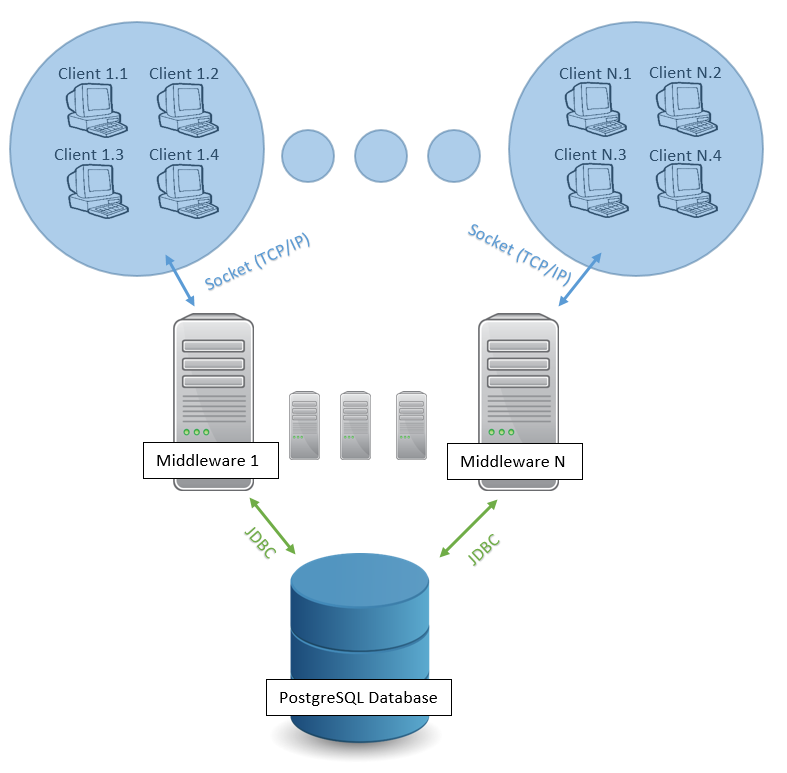
\includegraphics[width=0.7\linewidth]{figures/overall_design}
\caption{The overall system design}
\label{fig:overall_design}
\end{figure}
The detailed configurations of the machines are the following:
\begin{itemize}
	\item \textbf{Client}: The clients are runned on a C3.8xlarge machine. These machines provide 16 physical cores and thus allow a high number of processes to be executed concurrently.
	\item \textbf{Middleware}: The middlewares are runned on a C3.4xlarge machine. With their 8 physical cores they can nicely distribute the incoming read or write tasks onto the available threads.
	\item \textbf{Database}: The database is runned on a R3.4xlarge machine. Besides the 8 physical cores this machine type provides, it also is equiped with 122GB of RAM. This guarantees that also big tables can still fit into the working memory.
\end{itemize}

\subsection{Configuration and Deployment mechanisms}\label{sec:configuration-and-deployment-mechanisms}
In the scope of this project, I worked with two client machines, two middlewares and one database. The client deployment mechanism of the system was already introduced in section \ref{sec:workloads-and-deployment}. The deployment of the other two system parts follow the same schema:
\begin{itemize}
	\item \textbf{Deploy the Middleware}:
	\begin{enumerate}
		\item Enter the database IP into the corresponding field in \textit{ASL/config/config\_common.xml}
		\item Launch a middleware machine, install git and clone respository: Lookup steps (2) and (3) in section \ref{sec:workloads-and-deployment}
		\item Install all needed libraries and create necessary log folders:\newline
		\textit{sh /home/ec2-user/ASL/mw\_setup/setup\_middleware.sh}
		\item Start M middlewares on the current machine:\newline
		\textit{sh /home/ec2-user/ASL/mw\_setup/start\_middleware -n M}
		\item When the experiment is done hit ENTER to flush and close all logging files and shutdown gracefully
	\end{enumerate}
	\item \textbf{Deploy the Database}:
	\begin{enumerate}
		\item Launch a database machine and perform steps (2) and (3) of section \ref{sec:workloads-and-deployment}
		\item Setup, configure and run the database: \newline
		\textit{sh /home/ec2-user/ASL/db\_setup/setup\_database.sh}
		\item For control over the postgres process call \textit{/home/ec2-user/ASL/pg\_ctl command}, with \textit{command}, one of \{\textit{start}, \textit{stop}, \textit{status}, \textit{status}\}
	\end{enumerate}
\end{itemize}

\subsection{Logging and Benchmarking mechanisms}\label{sec:logging-and-benchmarking-mechanisms}
When done with the experiment it's important to fetch the data to the local machine fast and without much effort. This functionality is provided by \textit{ASL/download\_logs.sh}. Simply put the path of interest into the preconstructed command and then call it with like this: \textit{sh download\_logs.sh target\_folder}. Sometimes the data was too big to be plotted efficiently, so I built some log parsers which do some averaging or filtering on the data. This means more work, but also that I always could go back to the original data and be sure that I have anything I need for later computations. These parsers are implemented in Java and can be found in \textit{src/org/asl/experiments/baselines/database/logParser}. When the data was ready it was processed in Matlab where all plots are produces. The corresponding files are found in \textit{ASL/plotting tools}.

\section{Evaluation}\label{sec:evaluation}

Length: up to 10 pages

In this section we expect to see the different experiments you ran to
exercise the system, and with each experiment we expect a clear
description of the system configuration used, the hypothesis on behavior
and the explanation of the behavior observed (in terms of the different
design decisions taken beforehand) -- \emph{missing either of these for
an experiment might make you lose all points for that given experiment!}
Keep in mind that for a good explanation of the results of an experiment
you might have to use one or more methods of data analysis presented in
the lecture and in the book.

See below for a short description on what each part should contain.

\subsection{System Stability}\label{sec:system-stability}

To prove that your system functions correctly and that it is stable
include the trace of a 30 minute run, plotting both response time and
throughput. Use at least 30 clients (sending and receiving data), 2
middlewares and a non-empty database.
\TwoFig {figures/stability/stability_tp.eps} {Throughput behaviour} {fig:stability_tp}
		{figures/stability/stability_rt.eps} {Response time behaviour} {fig:stability_rt}
content length: 200, num db conns: 40, 120 clients on each 60 clients, 2 middlewares on each a seperate machine
\newline
workload was
send message, get queues with messages for client, read all messages of queue, read message from sender, remove top message from queue
\subsection{System Throughput}\label{sec:system-throughput}

Measure the maximum throughput of the system (describe the exact
configuration and workload, and the reasoning behind choosing these
particular ones) and show the average response time for this experiment.
\newline
since its not clear to me what exact configuration the maximum throughput yields, I let clients join dynamically the system. With this approach we can see how the throughput behaves with respect to the amount of clients in the system. The approach was to run each database connection number for 40 up to 120 clients, 10 clients joining every 20 seconds. msg size = 200, 2 middlewares.
the result is:
\begin{figure}[!htb]
\centering
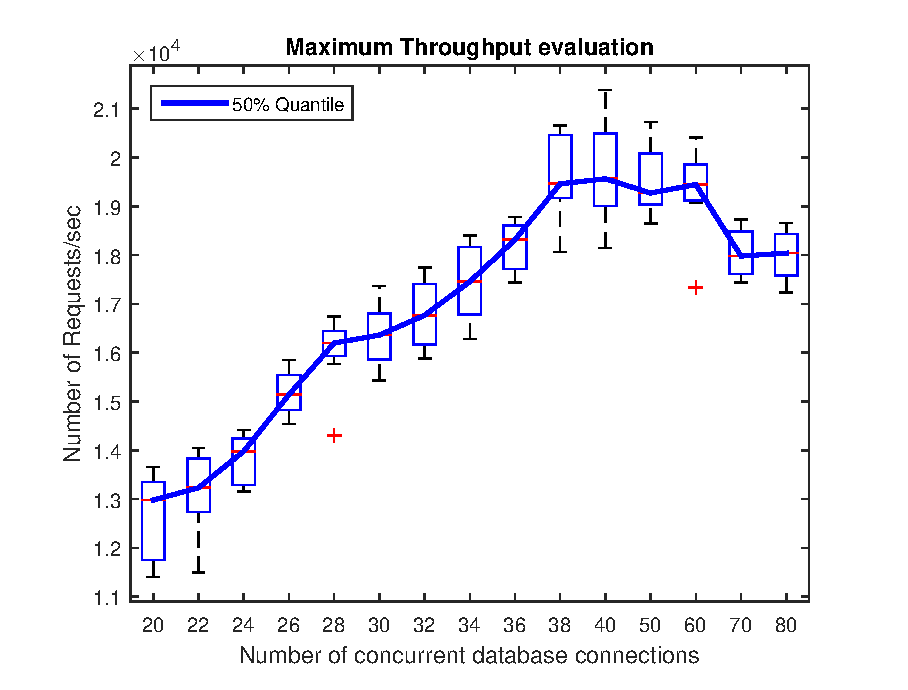
\includegraphics[width=0.7\linewidth]{figures/max_tp}
\caption{Maximum Throughput behaviour with respect to the number of database connections}
\label{fig:max_tp}
\end{figure}
The best possible configuration under this worload is with 60 clients, 40 database connections, 2 middlewares and a message size of 200.

\subsection{System Scalability}\label{sec:system-scalability}

Explain the different configurations used to explore the scalability of
your system, and the outcomes of these experiments in terms of
throughput and response times. The main goal of this subsection is to
define the ranges in which your system operates best.

\subsection{Response Time Variations}\label{sec:response-time-variations}

Report and analyze how the response times change in the system with
different message sizes, different number of clients and different
number of middleware nodes.

\subsection{$2^k$ Experiment}\label{sec:k-experiment}

Conduct a 2\^{}k analysis of your system (aim at exploring non-obvious
interactions of parameters). Use the methods learned in this lecture to
conduct the detailed analysis.

The \#Clients and \#DB Connections are evenly distributed over the middlewares if there are two in play.
\begin{landscape}
\begin{table}
\small
\centering
\caption{$2^k$ Factors}
\label{tbl:2k_labels}
\begin{tabular}{cccc}
	Symbol & Factor & Level -1 & Level 1 \\ \hline
	A & \#Middlewares & 1 & 2 \\
	B & \#Clients & 60 & 120 \\
	C & Message Length & 200 & 2000 \\
	D & \#DB Connections & 20 & 40 \\ \hline
\end{tabular}
\end{table}
\begin{table}[]
	\small
	\centering
	\caption{$2^k$ Effects}
	\label{tbl:2k}
	\begin{tabular}{|cccccccccccccccc|cc|}
		\hline
		I & A & B & C & D & AB & AC & AD & BC & BD & CD & ABC & ABD & ACD & BCD & ABCD & TP(Req/s) & RT(ms)\\ \hline
		1 & -1 & -1 & -1 & -1 & 1 & 1 & 1 & 1 & 1 & 1 & -1 & -1 & -1 & -1 & 1 & 12427 & 5.12\\
		1 & -1 & -1 & -1 & 1 & 1 & 1 & -1 & 1 & -1 & -1 & -1 & 1 & 1 & 1 & -1 & 14707 & 3.87 \\
		1 & -1 & -1 & 1 & -1 & 1 & -1 & 1 & -1 & 1 & -1 & 1 & -1 & 1 & 1 & -1 & 11859 & 4.84 \\
		1 & -1 & -1 & 1 & 1 & 1 & -1 & -1 & -1 & -1 & 1 & 1 & 1 & -1 & -1 & 1 & 16133 & 3.66 \\
		1 & -1 & 1 & -1 & -1 & -1 & 1 & 1 & -1 & -1 & 1 & 1 & 1 & -1 & 1 & -1 & 12413 & 9.98 \\
		1 & -1 & 1 & -1 & 1 & -1 & 1 & -1 & -1 & 1 & -1 & 1 & -1 & 1 & -1 & 1 & 18233 & 7.07 \\
		1 & -1 & 1 & 1 & -1 & -1 & -1 & 1 & 1 & -1 & -1 & -1 & 1 & 1 & -1 & 1 & 13238 & 9.14 \\
		1 & -1 & 1 & 1 & 1 & -1 & -1 & -1 & 1 & 1 & 1 & -1 & -1 & -1 & 1 & -1 & 16428 & 6.97 \\
		1 & 1 & -1 & -1 & -1 & -1 & -1 & -1 & 1 & 1 & 1 & 1 & 1 & 1 & -1 & -1 & 13488 & 4.69 \\
		1 & 1 & -1 & -1 & 1 & -1 & -1 & 1 & 1 & -1 & -1 & 1 & -1 & -1 & 1 & 1 & 15954 & 3.87 \\
		1 & 1 & -1 & 1 & -1 & -1 & 1 & -1 & -1 & 1 & -1 & -1 & 1 & -1 & 1 & 1 & 12289 & 4.94 \\
		1 & 1 & -1 & 1 & 1 & -1 & 1 & 1 & -1 & -1 & 1 & -1 & -1 & 1 & -1 & -1 & 15855 & 4.19 \\
		1 & 1 & 1 & -1 & -1 & 1 & -1 & -1 & -1 & -1 & 1 & -1 & -1 & 1 & 1 & 1 & 13017 & 9.16 \\
		1 & 1 & 1 & -1 & 1 & 1 & -1 & 1 & -1 & 1 & -1 & -1 & 1 & -1 & -1 & -1 & 17701 & 6.57 \\
		1 & 1 & 1 & 1 & -1 & 1 & 1 & -1 & 1 & -1 & -1 & 1 & -1 & -1 & -1 & -1 & 13054 & 9.31 \\
		1 & 1 & 1 & 1 & 1 & 1 & 1 & 1 & 1 & 1 & 1 & 1 & 1 & 1 & 1 & 1 & 12427 & 6.73 \\ \hline
		14650 & 221 & 561 & -91 & 1927 & -86 & -76 & -17 & -36 & 354 & 21 & 193 & 47 & 101 & -365 & 212 \\
		6.25 & -0.07 & 1.85 & -0.03 & -0.89 & -0.09 & 0.14 & 0.05 & -0.04 & -0.4 & 0.06 & 0.01 & -0.06 & -0.05 & 0.04 & -0.05
	\end{tabular}
\end{table}
\end{landscape}

\begin{table}
\centering
\caption{Variation explained by each factor in \% (Sum $\neq100$ due to rounding for better readability)}
\label{tbl:2k_labels}
\begin{tabular}{ccc}
	Parameter & TP & RT \\ \hline
	$q_{A}$ & 1.10  & 0.12  \\
	$q_{B}$ & \textbf{7.09} & \textbf{77.57}  \\
	$q_{C}$ & 0.19 & 0.03  \\
	$q_{D}$ & \textbf{83.35} & \textbf{17.80} \\
	$q_{AB}$ & 0.17 & 0.22  \\
	$q_{AC}$ & 0.13  & 0.47  \\
	$q_{AD}$ & 0.01  & 0.05  \\
	$q_{BC}$ & 0.03  & 0.04  \\
	$q_{BD}$ & 2.82  & 3.42 \\
	$q_{CD}$ & 0.01  & 0.07  \\
	$q_{ACB}$ & 0.84  & 0.00  \\
	$q_{ABD}$ & 0.05  & 0.08  \\
	$q_{ACD}$ & 0.23  & 0.05  \\
	$q_{BCD}$ & 3.99  & 0.03  \\
	$q_{ABCD}$ & 1.02  & 0.05  \\
\end{tabular}
\end{table}
It's clearly visible, that the throughput and response time are mainly dependent of each a single factor. For the throughput, the most important factor is the number of concurrent database connections (explains $\approx83.35\%$ of the variation). For the response time however the cruial factor is the number of active clients (explains $\approx77.57\%$ of the variation). In words this means the following:
\begin{itemize}
	\item \textbf{Throughput}: If more database connections are added, the throughput raises. If the number of database connections is reduces, also the throughput will decrease. The second important factor to consider is the number of clients operating concurrently in the whole system. With an effect of $561$ in column B (see table \ref{tbl:2k}), this yields, that when more clients join the system the throughput will go up, and vice-versa for less clients.
	\item \textbf{Response Time}: When more clients are join the system the response time will grow. If some clients leave the response time will decrease. The number of database connections has also nearly $\approx18\%$ of influence on the performance. Since the effect of $-0.89$ in the column D (see table \ref{tbl:2k}) is negative, this means, that the more connections to the database are available, the smaller the response will be, and vice-versa for less connections to the database.
\end{itemize}
\subsection{Conclusion}\label{sec:conclusion}

To conclude the report summarize the behavior of the system in terms of
the design and the representative workloads. Finally, outline in a few
points what would you do differently if you could design the system
anew.


\end{document}
